\subsection{$\pi$- \& $\sigma$-orbitaler}

Da vi så de atomare orbitaler gav vi dem navnene, s,p,d og f. Molekylære orbitaler har også navne, men jeg vil i denne opgave primært have fokus på hhv. $\pi$-orbitaler og $\sigma$-orbitaler. Vi betragter et eksempel med et homonukleært diatomisk molekyle som $H_2$. De to hydrogenatomer der er bundet sammen har hver deres egen elektron, men når de er sig tilpas tæt nok på hinanden vil elektronerne mere eller mindre befinde sig mellem de to kerner. Da elektronerne er negativt ladede og de 2 hydrogenkerner er positivt ladede, vil elektronerne blive tiltrukket af begge kerner og have et lavere niveau af energi end de ville have isolerede (MANGLER NOTE GENERAL CHEMISTRY SIDE 150). Da elektronerne søger at have en så lav energi som muligt vil de befinde sig mellem de to kerner og stabilisere molekylet. Denne slags orbitaler kaldes \textbf{bindende} orbitaler, da de som navnet antyder binder molekylet sammen. På figur 4 er det illustreret hvordan to atomare orbitaler går sammen om at danne en bindende $\sigma_s$ orbital. 
\begin{center}
\begin{figure}[ht!]
  \centering
  \begin{tikzpicture}[scale=2]
  \begin{scope}[font=\itshape]% 

  \draw[-latex] (0,-1)--(0,1) node[above]{Stigende energi};
  \orbital[color = purple, opacity = 1, scale = 2, pos = {(1,0.65)}]{s} 
  \orbital[color = purple, opacity = 1, scale = 2, pos = {(2,0.65)}]{s} 
  \node[above] at (1,0.5) {+};  
  \node[above] at (2,0.5) {+};
  \node[above] at (1,0) {s orbital};
  \node[above] at (2,0) {s orbital};
	\draw[-latex] (2.5,0.65)--(3.5,-0.10);
 		
 		
 		
 \orbital[color = purple, opacity = 0.2, scale = 2, pos = {(4,-0.5)}]{s} 
  \orbital[color = purple, opacity = 0.3, scale = 2, pos = {(4.5,-0.5)}]{s}  	
  	
  \node[above] at (4.2,-1.5) {Bindende orbital $\sigma_s$};
 	\node[above] at (4,-0.65) {+}; 
 	\node[above] at (4.5,-0.65) {+}; 
  \end{scope}

  \begin{pgfonlayer}{backbackground}
  \fill[white](current bounding box.south west)rectangle
  (current bounding box.north east);
  \end{pgfonlayer}
  \end{tikzpicture}
  \caption{1s orbital} \end{figure}
	\end{center}
	
Denne bindende $\sigma$-orbital er faktisk det vi også kender som en $\sigma$-binding eller en kovalent binding. Kovalente bindinger er netop defineret som molekylære bindinger, der involverer at to atomer deler deres elektroner. 
\\

På samme måde som med $\sigma$-orbitalerne dannes $\pi$-orbitalerne ved, at to atomers befinder sig tæt på hinanden og elektronerne kan få en lavere energi ved at befinde sig i det sted hvor orbitalerne overlapper. $\pi$-orbitalerne adskiller sig alligevel fra $\sigma$-orbitalerne ved ikke at kunne blive dannet af overlap mellem s-orbitaler. En illustration af hvordan $\pi$-bindinger dannes ved et overlap af p-orbitaler: se figur 5. 

\begin{center}
\begin{figure}[ht!]
  \centering
  \begin{tikzpicture}[scale=2]
  \begin{scope}[font=\itshape]% 

  \draw[-latex] (-0.5,-1)--(-0.5,1) node[above]{Stigende energi};
  \orbital[pcolor = purple, opacity = 1, scale = 1, pos = {(1,0.65)}]{pz} 
  \orbital[pcolor = purple, opacity = 1, scale = 1, pos = {(2,0.65)}]{pz} 
  \node[above] at (0.8,-0.40) {$p_z-orbital$};
  \node[above] at (2.2,-0.40) {$p_z-orbital$};
	\draw[-latex] (2.5,0.65)--(3.5,-0.10);
  \node[above] at (1,0.5) {+};
  \node[above] at (2,0.5) {+};
 		
 \orbital[color = purple, opacity = 1, scale = 2, pos = {(4,-0.5)}]{s} 
  \orbital[color = purple, opacity = 1, scale = 2, pos = {(4.5,-0.5)}]{s}  	
  
 \orbital[color = lightgray, opacity = 0.3, scale = 2, pos = {(4,-1)}]{s} 
  \orbital[color = lightgray, opacity = 0.3, scale = 2, pos = {(4.5,-1)}]{s}  	  
  	
  \node[above] at (4.2,-2) {Bindende orbital $\pi_p$};
 		
 		
  \node[above] at (4,-0.90) {+};
  \node[above] at (4.5,-0.90) {+};		
 		
  \end{scope}

  \begin{pgfonlayer}{backbackground}
  \fill[white](current bounding box.south west)rectangle
  (current bounding box.north east);
  \end{pgfonlayer}
  \end{tikzpicture}
  \caption{1s orbital} \end{figure}
	\end{center}
\pagebreak
	
Nu har vi set på både $\sigma$-orbitaler /bindinger og $\pi$-orbitaler / bindinger - men hver for sig. Hvis de to orbitaler eksisterer sammentidigt i et molekyle har vi faktisk en dobbeltbinding. Dobbeltbindinger er netop en $\sigma$- og en $\pi$-binding. Illustret som en tegning ville det se ud på følgende måde, se Figur 6: 

\begin{center}
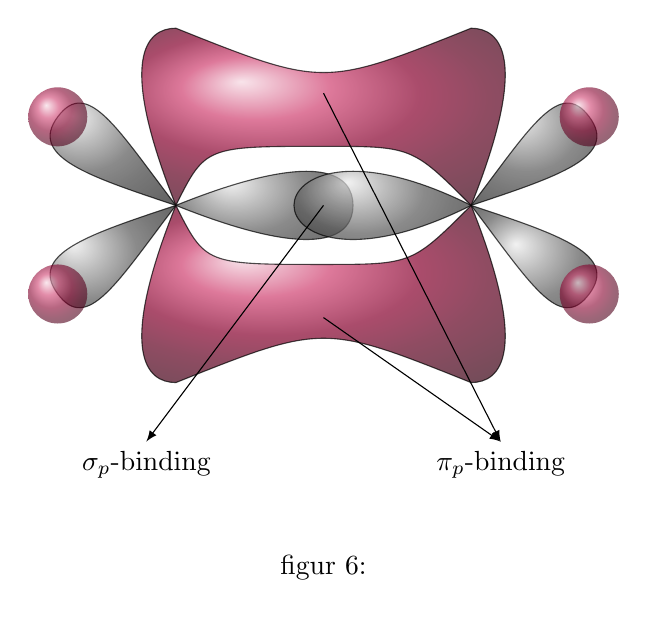
\begin{tikzpicture}[scale=0.75]

\shade[shading=ball, ball color=gray,draw,opacity=.7] (-2.5,0) .. controls (0,1) and     (.5,0.5) .. (.5,0)
.. controls (.5,-.5) and (0,-1) .. (-2.5,0);

\shade[shading=ball, ball color=gray,draw,opacity=.7] (2.5,0) .. controls (.5,1) and     (-.5,0.5) .. (-.5,0)
.. controls (-.5,-.5) and (.5,-1) .. (2.5,0);


\shade[shading=ball, ball color=gray,draw,opacity=.7] (-2.5,0) .. controls (-4,0.5) and     (-5,0.83) .. (-4.5,1.5)
.. controls (-4,2.17) and (-3.5,1.31) .. (-2.5,0);

\shade[shading=ball, ball color=gray,draw,opacity=.7] (-2.5,0) .. controls (-4,-0.5)     and (-5,-0.83) .. (-4.5,-1.5)
.. controls (-4,-2.17) and (-3.5,-1.31) .. (-2.5,0);


\shade[shading=ball, ball color=gray,draw,opacity=.7] (2.5,0) .. controls (4,0.5) and     (5,0.83) .. (4.5,1.5)
.. controls (4,2.17) and (3.5,1.31) .. (2.5,0);

\shade[shading=ball, ball color=gray,draw,opacity=.7] (2.5,0) .. controls (4,-0.5) and     (5,-0.83) .. (4.5,-1.5)
.. controls (4,-2.17) and (3.5,-1.31) .. (2.5,0);

\shade[shading=ball, ball color=purple,opacity=0.6] (4.5,1.5) circle (0.5);

\shade[shading=ball, ball color=purple,opacity=0.6] (4.5,-1.5) circle (.5);

\shade[shading=ball, ball color=purple,opacity=0.6] (-4.5,-1.5) circle (.5);

\shade[shading=ball, ball color=purple,opacity=0.6] (-4.5,1.5) circle (.5);


\shade[shading=ball, ball color=purple,draw,opacity=.7] (-2.5,0) .. controls (-3.5,2.5)     and (-3,3) .. (-2.5,3)
.. controls (0,2) .. (2.5,3)
.. controls (3,3) and (3.5,2.5) .. (2.5,0)
.. controls (1.5,1) .. (0,1)
.. controls (-2,1) .. (-2.5,0);


\shade[shading=ball, ball color=purple,draw,opacity=.7] (-2.5,0) .. controls (-3.5,-2.5)     and (-3,-3) .. (-2.5,-3)
.. controls (0,-2) .. (2.5,-3)
.. controls (3,-3) and (3.5,-2.5) .. (2.5,-0)
.. controls (1.5,-1) .. (0,-1)
.. controls (-2,-1) .. (-2.5,-0);

\draw[-latex] (0,0)--(-3,-4) node[below]{$\sigma_p$-binding};

\draw[-latex] (0,1.9)--(3,-4) node[below]{$\pi_p$-binding};

\draw[-latex] (0,-1.9)--(3,-4) node[below]{ };


\node[above] at (0,-6.5){figur 6: };
\end{tikzpicture}
\end{center}

$\sigma$-bindingerne er de stærkestee af de kovalente bindinger. Dernæst kommer $\pi$-bindingerne. blabla MO teori...


Det er nemmelig ikke alle atomer, der har mulighed for at danne kovalente bindinger imellem sig. Når 2 atomer går sammen om at danne en kovalent binding er det fordi, at de hver især er ustabile. At de er ustabile er ens betydende med, at de ikke har deres orbitaler af højeste energiniveau fyldt ud. Hver orbital vil gerne have en spin-op og en spin-ned elektron. Når nogle atomer så alligevel ikke vælger at gå sammen og danne en kovalent binding er det enten fordi, at de har for mange mange elektroner til, at de kun kan befinde sig mellem atomerne og danne en bindende $\sigma$-binding og derfor befinder sig i en orbital, der kræver et højere energiniveau og derfor er anti-bindende. 
